% \input{\pSections "sec-spreadsheet"}

\section{Writ Large}

Radar is an invaluable tool for space domain awareness which can characterize not only location, but also orientation of satellites in space. It can answer where antennas are pointed and how a space craft is maneuvering. The open question is one of interpreting the radar return section. The key value is the amount of energy returned by reflection, and this is the essence of the radar cross section (res).

Figure \ref{fig:wiki} shows a sample radar cross section measurement for a vintage A-26 Invader. The strength of the return signal varies over several orders of magnitude depending upon the viewing angle.

\begin{figure}[htbp]
\begin{center}
	\href{https://en.wikipedia.org/wiki/Radar_cross_section#/media/File:Sigma_invader_RCS.png}{
		\includegraphics[ width = 3in ]{\pLocalGraphics Sigma_invader_RCS.png} }
\caption{A radar cross section measurement for the A-26 Invader taken from the Wikipedia article on \href{https://en.wikipedia.org/wiki/Radar_cross_section}{Radar Cross Section} show energy change where 0 db represents 1 milliwatt return energy.}
\label{fig:wiki}
\end{center}
\end{figure}

A simplified aircraft model in figure \ref{fig:toy} presents requisite variation without over-complications and makes the point that even a stealthy aircraft can present large cross sections at proper view angles as seen in table \ref{tab:views}.
\begin{figure}[htbp] 
   \centering
   \includegraphics[ width=4in ]{\pLocalGraphics b20-glamor} 
   \caption{Toy model for aircraft. Although simplistically rendered, this representation is adequate for over the horizon radars.}
   \label{fig:toy}
\end{figure}

Look angle
\begin{table}[htp]
\begin{center}
\begin{tabular}{c}
	\includegraphics[ width=3in ]{\pLocalGraphics b20-above} \\
	\includegraphics[ width=3in ]{\pLocalGraphics b20-side} \\
	\includegraphics[ width=3in ]{\pLocalGraphics b20-nose} \\
\end{tabular}
\end{center}
\caption{Different aircraft views present very different cross-sectional areas.}
\label{tab:views}
\end{table}%

The purpose of this analysis is to start with a CAD model of a structure and simulate the radar cross section, a sample show in figure \ref{fig:mural}.
\begin{figure}[htbp] 
   \centering
   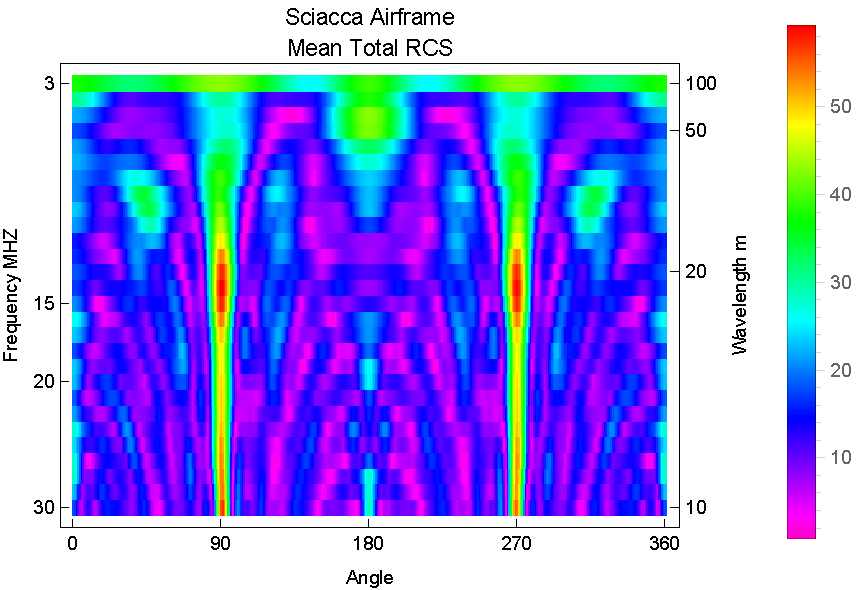
\includegraphics[ width=4in ]{\pLocalGraphics fits/Sciacca Airframe rcs.pdf} 
   \caption{Output for a radar backscatter simulation for radar frequencies from $3 - 30$ MHz, corresponding to wavelengths of $10-100$ m.}
   \label{fig:mural}
\end{figure}

 render the radar cross section into a form like
	\begin{equation*}
		\begin{split}
			\sigma_{3}\paren{\theta} &= 35.237 \pm 0.012   +  (1.675 \pm 0.018) \cos \theta  +  (-3.434 \pm 0.018) \cos 2\theta  +  (-0.866 \pm 0.018) \cos 3\theta   \\
			&+  (5.386 \pm 0.018) \cos 4\theta  +  (-1.280 \pm 0.018) \cos 5\theta  +  (1.379 \pm 0.018) \cos 6\theta +   (-0.675 \pm 0.018) \cos 7\theta
		\end{split}
	\end{equation*}	
where $\theta$ is an azimuthal angle with $\theta=0$ representing a nose-one view and $\pm \pi representing a tail-on view$


%     %     %     %     %     %     %     %     %
\subsection{Toy Satellite Model}
A toy satellite model is much easier to start with for developing a data analysis can reduction chain. The model below (figure /ref{tab:toy-sat}) features a spherical body and readily distinguishable solar panels.
\begin{figure}[htbp]
\begin{center}
		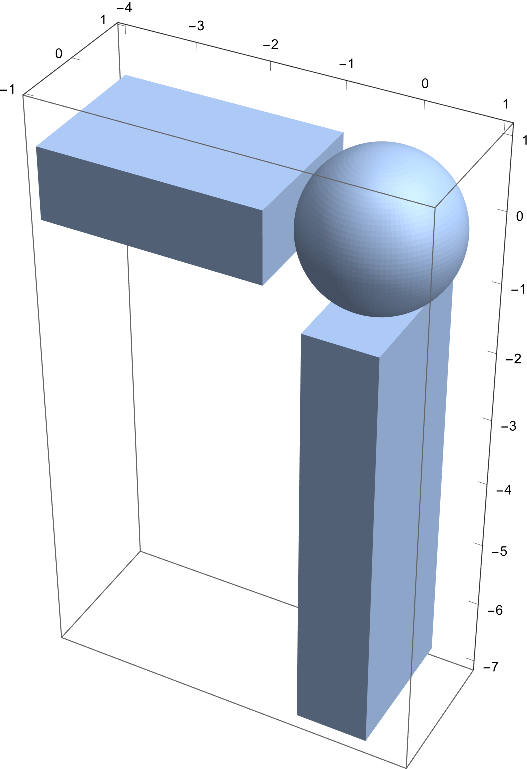
\includegraphics[ width = 2.5in ]{\pLocalGraphics proto/full} 
\caption{A toy satellite model designed to present a spherical backscatter and resonances at 6, 3, 2, and 1 meter wavelengths.}
\label{tab:toy-sat}
\end{center}
\end{figure}

\begin{table}[htp]
\caption{Contrasting views of a toy satellite present very different cross sectional areas, $A$.}
\begin{center}
\begin{tabular}{ccc}
		$A \approx \paren{\pi  + 12}r^{2}$ & $A = \paren{\pi  + 9}r^{2}$ & $A \approx \paren{\pi  + 6}r^{2}$ \\\hline
		
\includegraphics[ width = 1in ]{\pLocalGraphics proto/satI00}  & 
		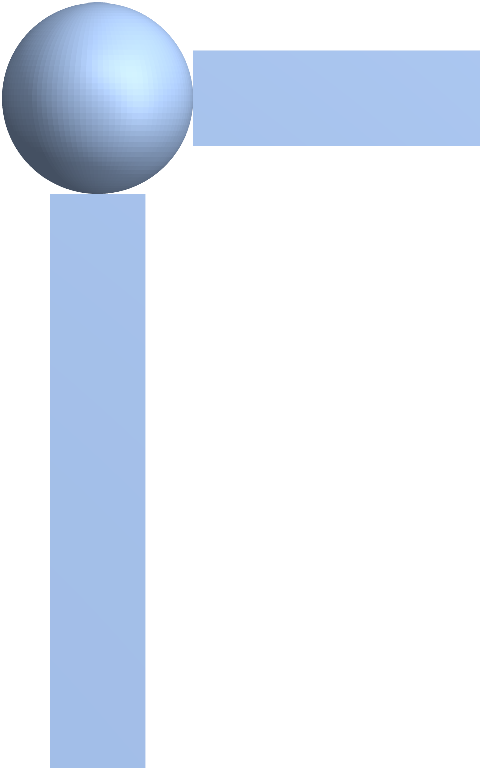
\includegraphics[ width = 2.5in ]{\pLocalGraphics proto/sat0I0}   &
		\raisebox{3in}{
\includegraphics[ width = 2.5in ]{\pLocalGraphics proto/sat00I}} 	\\
\end{tabular}
\end{center}
\label{tab:views}
\end{table}%



\endinput  %  ==  ==  ==  ==  ==  ==  ==  ==  ==
